\documentclass[tikz,border=6pt]{standalone}
\usetikzlibrary{arrows.meta,positioning,calc}
\makeatletter
\AtBeginDocument{\global\let\pgf@selectfontorig\relax}
\makeatother

\newcommand{\interleave}[1]{\mathbin{{|\!|\!|}_{#1}}}

\tikzset{
  nodebox/.style={draw=black, rounded corners=4pt, very thick, fill=gray!4,
    minimum width=10mm, minimum height=7mm, align=center, inner sep=2pt},
  initial/.style={-Latex, very thick},
  edge/.style={-Latex, thick, shorten >=1pt, shorten <=1pt},
  labelbox/.style={inner sep=5pt}
}

\newcommand{\initarrow}[2]{\draw[initial] #1 -- (#2);}

\begin{document}
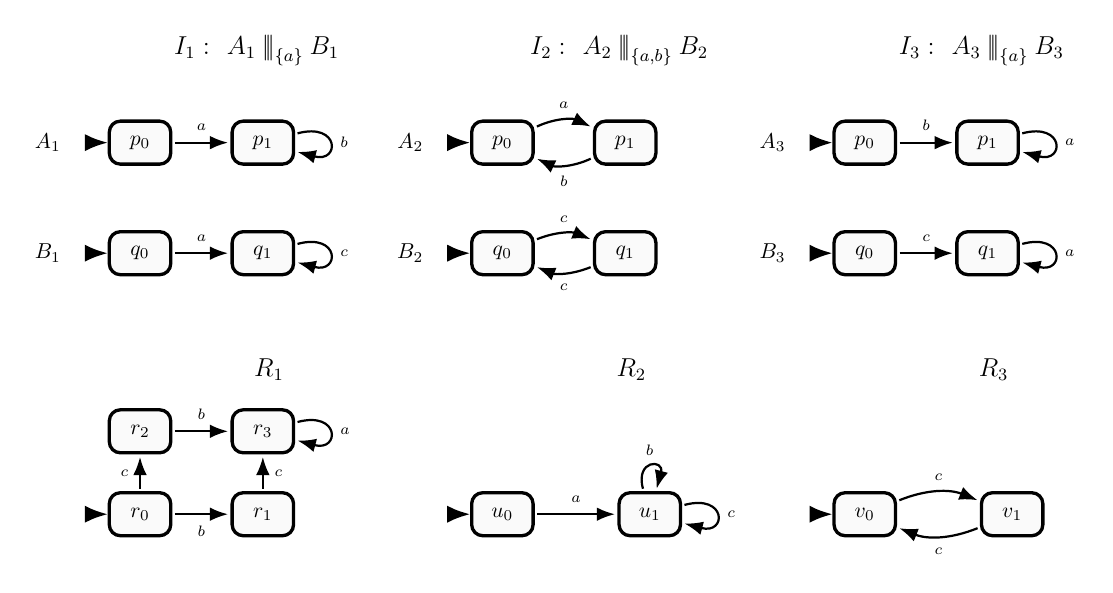
\begin{tikzpicture}[scale=.78, transform shape]
  \begin{scope}[shift={(0,5.2)}]
    \node at (1.9,2.35) {\bfseries\large $I_1:\ A_1 \interleave{\{a\}} B_1$};
    \node at (-1.5,.85) {$A_1$};
    \node[nodebox] (a10) at (0,.85) {$p_0$};
    \node[nodebox] (a11) at (2,.85) {$p_1$};
    \initarrow{(-.65,.85)}{a10.west}
    \draw[edge] (a10) -- node[labelbox,above] {\scriptsize $a$} (a11);
    \draw[edge,loop right,looseness=7] (a11) to node[labelbox,right] {\scriptsize $b$} (a11);
    \node at (-1.5,-.95) {$B_1$};
    \node[nodebox] (b10) at (0,-.95) {$q_0$};
    \node[nodebox] (b11) at (2,-.95) {$q_1$};
    \initarrow{(-.65,-.95)}{b10.west}
    \draw[edge] (b10) -- node[labelbox,above] {\scriptsize $a$} (b11);
    \draw[edge,loop right,looseness=7] (b11) to node[labelbox,right] {\scriptsize $c$} (b11);
  \end{scope}

  \begin{scope}[shift={(5.9,5.2)}]
    \node at (1.9,2.35) {\bfseries\large $I_2:\ A_2 \interleave{\{a,b\}} B_2$};
    \node at (-1.5,.85) {$A_2$};
    \node[nodebox] (a20) at (0,.85) {$p_0$};
    \node[nodebox] (a21) at (2,.85) {$p_1$};
    \initarrow{(-.65,.85)}{a20.west}
    \draw[edge,bend left=25] (a20) to node[labelbox,above] {\scriptsize $a$} (a21);
    \draw[edge,bend left=25] (a21) to node[labelbox,below] {\scriptsize $b$} (a20);
    \node at (-1.5,-.95) {$B_2$};
    \node[nodebox] (b20) at (0,-.95) {$q_0$};
    \node[nodebox] (b21) at (2,-.95) {$q_1$};
    \initarrow{(-.65,-.95)}{b20.west}
    \draw[edge,bend left=22] (b20) to node[labelbox,above] {\scriptsize $c$} (b21);
    \draw[edge,bend left=22] (b21) to node[labelbox,below] {\scriptsize $c$} (b20);
  \end{scope}

  \begin{scope}[shift={(11.8,5.2)}]
    \node at (1.9,2.35) {\bfseries\large $I_3:\ A_3 \interleave{\{a\}} B_3$};
    \node at (-1.5,.85) {$A_3$};
    \node[nodebox] (a30) at (0,.85) {$p_0$};
    \node[nodebox] (a31) at (2,.85) {$p_1$};
    \initarrow{(-.65,.85)}{a30.west}
    \draw[edge] (a30) -- node[labelbox,above] {\scriptsize $b$} (a31);
    \node at (-1.5,-.95) {$B_3$};
    \node[nodebox] (b30) at (0,-.95) {$q_0$};
    \node[nodebox] (b31) at (2,-.95) {$q_1$};
    \initarrow{(-.65,-.95)}{b30.west}
    \draw[edge] (b30) -- node[labelbox,above] {\scriptsize $c$} (b31);
    \draw[edge,loop right,looseness=7] (a31) to node[labelbox,right] {\scriptsize $a$} (a31);
    \draw[edge,loop right,looseness=7] (b31) to node[labelbox,right] {\scriptsize $a$} (b31);


  \end{scope}

  \begin{scope}[shift={(0,0)}]
    \node at (2.1,2.35) {\bfseries\large $R_1$};
    \node[nodebox] (r100) at (0,0) {$r_0$};
    \node[nodebox] (r110) at (2,0) {$r_1$};
    \node[nodebox] (r101) at (0,1.35) {$r_2$};
    \node[nodebox] (r111) at (2,1.35) {$r_3$};
    \initarrow{(-.75,0)}{r100.west}
    \draw[edge] (r100) -- node[labelbox,below] {\scriptsize $b$} (r110);
    \draw[edge] (r100) -- node[labelbox,left] {\scriptsize $c$} (r101);
    \draw[edge] (r101) -- node[labelbox,above] {\scriptsize $b$} (r111);
    \draw[edge] (r110) -- node[labelbox,right] {\scriptsize $c$} (r111);
    \draw[edge,loop right,looseness=7] (r111) to node[labelbox,right] {\scriptsize $a$} (r111);

  \end{scope}

  \begin{scope}[shift={(5.9,0)}]
    \node at (2.1,2.35) {\bfseries\large $R_2$};
    \node[nodebox] (r200) at (0,0) {$u_0$};
    \node[nodebox] (r211) at (2.4,0) {$u_1$};
    \initarrow{(-.75,0)}{r200.west}
    \draw[edge] (r200) -- node[labelbox,above] {\scriptsize $a$} (r211);
    \draw[edge,loop above,looseness=7] (r211) to node[labelbox,above] {\scriptsize $b$} (r211);
    \draw[edge,loop right,looseness=7] (r211) to node[labelbox,right] {\scriptsize $c$} (r211);
  \end{scope}

  \begin{scope}[shift={(11.8,0)}]
    \node at (2.1,2.35) {\bfseries\large $R_3$};
    \node[nodebox] (r300) at (0,0) {$v_0$};
    \node[nodebox] (r301) at (2.4,0) {$v_1$};
    \initarrow{(-.75,0)}{r300.west}
    \draw[edge,bend left=22] (r300) to node[labelbox,above] {\scriptsize $c$} (r301);
    \draw[edge,bend left=22] (r301) to node[labelbox,below] {\scriptsize $c$} (r300);
  \end{scope}
\end{tikzpicture}
\end{document}
